\documentclass{article}
\usepackage{listings}
\usepackage{xcolor}
\usepackage{caption}
\usepackage{graphicx, subfig}
\usepackage{float}
\usepackage[utf8]{inputenc}
\usepackage{fontspec}
\setmonofont{Sarasa-Mono-Slab-SC-Regular}

\lstset{
basicstyle=\ttfamily\scriptsize,
numbers=none,
breaklines,%自动换行
columns=flexible,%不随便添加空格,只在已经有空格的地方添加空格
keywordstyle=\color{blue}, %设置关键字颜色
        commentstyle=\color[cmyk]{1,0,1,0}, %设置注释颜色
numberstyle=\tiny,
frame=shadowbox,
rulesepcolor=\color{red!20!green!20!blue!20},
escapeinside=`', %将中文放在`和'之间,可以在lstlisting环境中准确的显示中文
}

\title{Assignment 2}
\author{Wangzhihui Mei, HongYi Huang, ChangXu, Zijia He}
\date{November 2020}

\begin{document}

\maketitle
\section{Task1}
\subsection{data describe}
\setlength{\parindent}{0pt}
Cardiovascular diseases (CVDs) is the leading cause of mortality in India. Ischemic heart disease and stroke are the predominant causes and are responsible for nearly 80\% of CVD deaths. 

\begin{lstlisting}[language=R]
dt <- read.csv("heart1.csv",na.strings = "?")
dt <- na.omit(dt) # handle NA
head(dt)
\end{lstlisting} 

\begin{figure}[H]
  \centering
  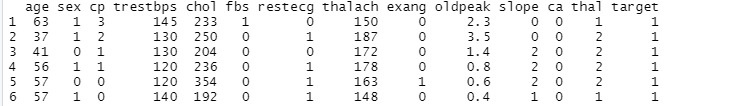
\includegraphics[width=1\textwidth]{task1_1_dtHead.png} %1.png是图片文件的相对路径
\end{figure}

This database contains 14 attributes. The "target" field refers to the presence of CVD in the patient. It is
integer valued 0 (no presence) or 1 (presence). Next we look in detail at the data characteristics of each attribute.
\\
Age: Age in years\\
Sex: (1 = male; 0 = female)\\
CP:Chest pain type(1-typical angina, 2-atypical angina, 3-non-anginal	pain, 4-asymptomatic )\\
trestbps:Resting blood pressure (in mm Hg on admission to the hospital)\\
Chol:Serum cholestoral in mg/dl\\
Fbs:Indicator of whether fasting blood sugar>120 mg/dl (1-true; 0-false)\\
restecg:Resting electrocardiographic results\\
exang:Exercise induced angina (1-yes; 0-no)\\
oldpeak:ST depression induced by exercise relative to rest\\
slope:Slope of the peak exercise ST segment (1-upsloping, 2-flat, 3-downsloping)\\
ca:Number of major vessels (0-3) colored by flourosopy\\
thal:Summary of heart condition(3 = normal, 6 = fixed defect, 7=reversable defect)\\
target:the “The Disease Diagnosis” field refers to the presence of heart disease in the patient(0-No presence,1-Presence) 
\begin{lstlisting}[language=R]
  summary(dt)
\end{lstlisting} 
  
  \begin{figure}[H]
    \centering
    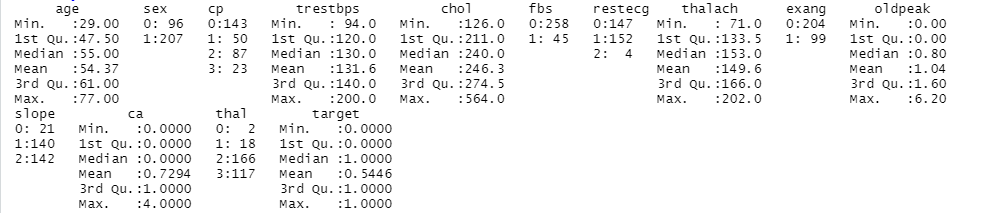
\includegraphics[width=1\textwidth]{task1_1_dtSummary.png}
  \end{figure}

\subsection{logistic regression}
By looking at the details of each data item in the dataset, it was found that the values of age as well as maximum heart rate were quite different and needed to be processed for both data items.
\begin{lstlisting}[language=R]
summary(dt$age)
dt$age<-cut(as.numeric(dt$age),breaks=3,labels=c("low1","normal1","high1"))
levels(dt$age)
table(dt$age)
\end{lstlisting}
\begin{figure}[H]
  \centering
  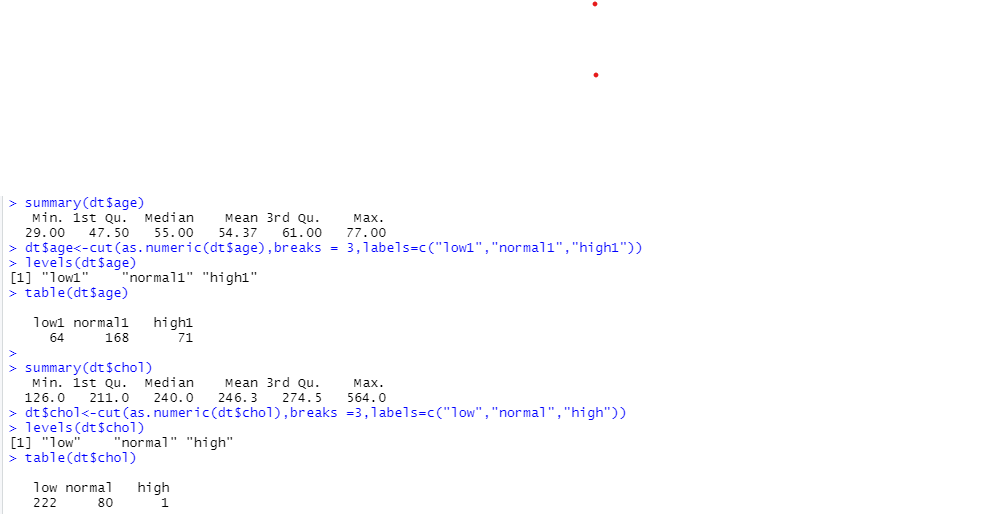
\includegraphics[width=1\textwidth]{task1_1_ageSummary.png}
\end{figure}
Dividing the data set into training and test sets according to a 7 to 3 ratio
% \begin{figure}[H]
%   \centering
%   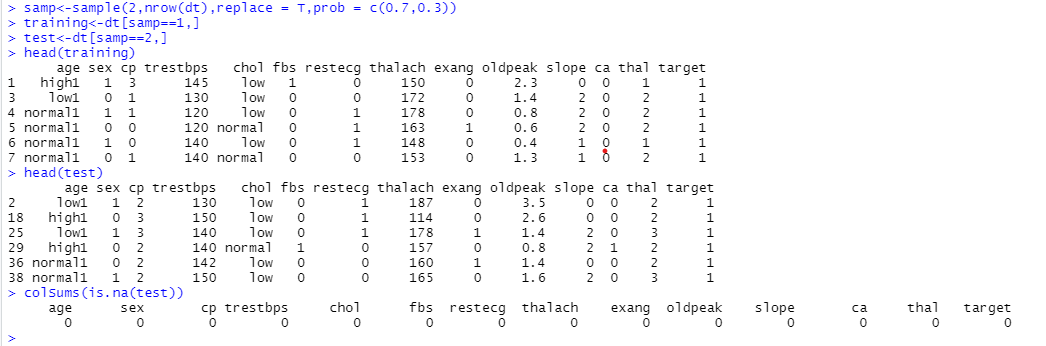
\includegraphics[width=1\textwidth]{task1_1_dataDivide.png}
% \end{figure}
\clearpage
\begin{lstlisting}[language=R]
  dt <- read.csv("heart1.csv",na.strings = "?")
  dt <- na.omit(dt) # handle NA
  head(dt)
  age sex cp trestbps chol fbs restecg thalach exang oldpeak slope ca thal target
  1  63   1  3      145  233   1       0     150     0     2.3     0  0    1      1
  2  37   1  2      130  250   0       1     187     0     3.5     0  0    2      1
  3  41   0  1      130  204   0       0     172     0     1.4     2  0    2      1
  4  56   1  1      120  236   0       1     178     0     0.8     2  0    2      1
  5  57   0  0      120  354   0       1     163     1     0.6     2  0    2      1
  6  57   1  0      140  192   0       1     148     0     0.4     1  0    1      1
  \end{lstlisting}
Next, a logistic regression prediction model is built using the training set data
\begin{figure}[H]
  \centering
  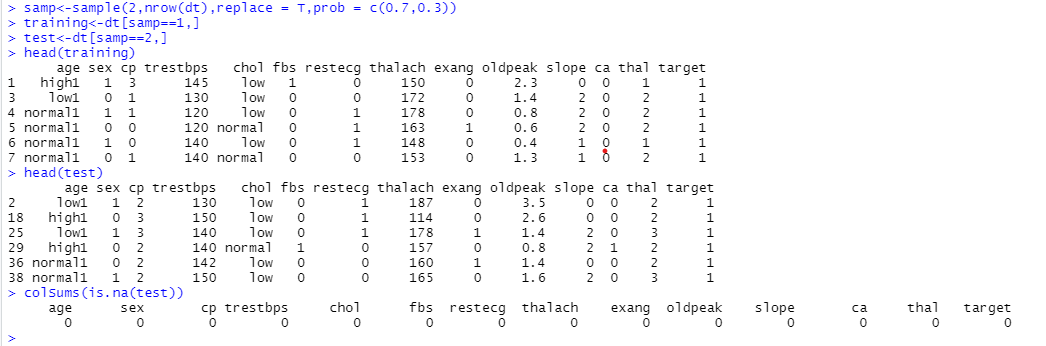
\includegraphics[width=1\textwidth]{task1_1_dataDivide.png}
\end{figure}

\begin{lstlisting}[language=R]
> mod<-glm(target~.,data = training,family = binomial('logit'))
> summary(mod)

Call:
glm(formula = target ~ ., family = binomial("logit"), data = training)

Deviance Residuals: 
    Min       1Q   Median       3Q      Max  
-2.6397  -0.3260   0.1472   0.4614   2.4521  

Coefficients:
              Estimate Std. Error z value Pr(>|z|)   
(Intercept)    1.43597    3.14892   0.456  0.64838   
agenormal1    -1.08551    0.66165  -1.641  0.10088   
agehigh1       0.19073    0.82340   0.232  0.81682   
sex1          -1.27014    0.63533  -1.999  0.04559 * 
cp1            1.07789    0.64981   1.659  0.09716 . 
cp2            1.76202    0.59697   2.952  0.00316 **
cp3            2.33462    0.87380   2.672  0.00754 **
trestbps      -0.02011    0.01359  -1.480  0.13899   
cholnormal    -0.87024    0.56281  -1.546  0.12204   
cholhigh      13.46342 1455.39800   0.009  0.99262   
fbs1           1.40058    0.78331   1.788  0.07377 . 
restecg1       0.75994    0.47349   1.605  0.10850   
restecg2       0.18667    3.24270   0.058  0.95409   
thalach        0.01516    0.01288   1.177  0.23910   
exang1        -1.06170    0.53172  -1.997  0.04585 * 
oldpeak       -0.52696    0.26619  -1.980  0.04774 * 
slope1        -0.74014    1.04764  -0.706  0.47989   
slope2         0.01442    1.13336   0.013  0.98985   
ca            -0.57276    0.23372  -2.451  0.01426 * 
thal1          1.48527    2.16992   0.684  0.49367   
thal2          1.70341    1.83567   0.928  0.35343   
thal3          0.18380    1.87081   0.098  0.92174   
---
Signif. codes:  0 ‘***’ 0.001 ‘**’ 0.01 ‘*’ 0.05 ‘.’ 0.1 ‘ ’ 1

(Dispersion parameter for binomial family taken to be 1)

    Null deviance: 292.99  on 213  degrees of freedom
Residual deviance: 134.65  on 192  degrees of freedom
AIC: 178.65

Number of Fisher Scoring iterations: 14
\end{lstlisting} 
After getting the training model, we need to evaluate the suitability of the model for the scenario by the following metrics
\begin{lstlisting}[language=R]
  predicted<-predict(mod,training,type ="response")
  training$predd<-round(predicted,3)
  View(training)
  ggplot( training, aes( training$predd, color = as.factor(training$target) ) ) + 
    geom_density( ) +
    ggtitle( "Training Set's Predicted Score" )
  training$predw<-ifelse(training$predd>0.46,1,0)
\end{lstlisting}
\begin{figure}[H]
  \centering
  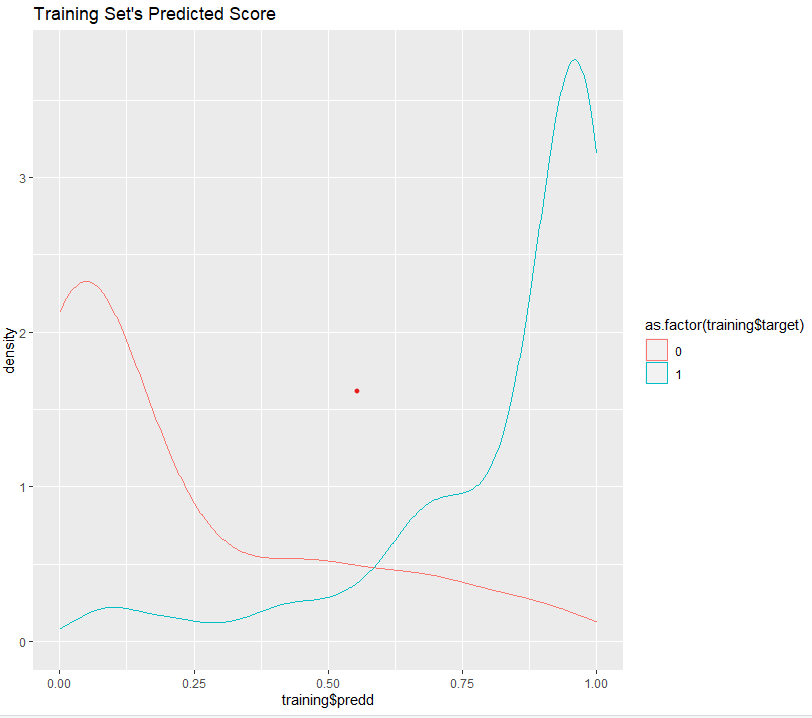
\includegraphics[width=1\textwidth]{task1_1_preScore.png}
\end{figure}

\begin{lstlisting}[language=R]
> training$predw<-ifelse(training$predd>0.46,1,0)
> confusn<-confusionMatrix(training$target,training$predw,threshold = 0.46)
> confusn
   0   1
0 74  11
1 19 110
> confusn<-as.matrix(confusn)
> AccuracyRate <- sum(diag(confusn))/sum(confusn)
> AccuracyRate
[1] 0.8598131
\end{lstlisting}
Similarly, we need to evaluate this model in the test set
\begin{lstlisting}[language=R]
> test$prob <- predict(mod,test,type = "response")
> View(test)
> ggplot( test, aes( test$prob, color = as.factor(test$target) ) ) + geom_density( size = 1 ) + ggtitle( "Test Set's Predicted Score" )
> test$predc<-ifelse(test$prob>0.475,1,0)
> confusn<-confusionMatrix(test$target,test$predc,threshold = 0.475)
> confusn
   0  1
0 31  7
1 14 37
> class(confusn)
[1] "data.frame"
> confusn<-as.matrix(confusn)
> AccuracyRate <- sum(diag(confusn))/sum(confusn)
> AccuracyRate
[1] 0.7640449
\end{lstlisting}
\begin{figure}[H]
  \centering
  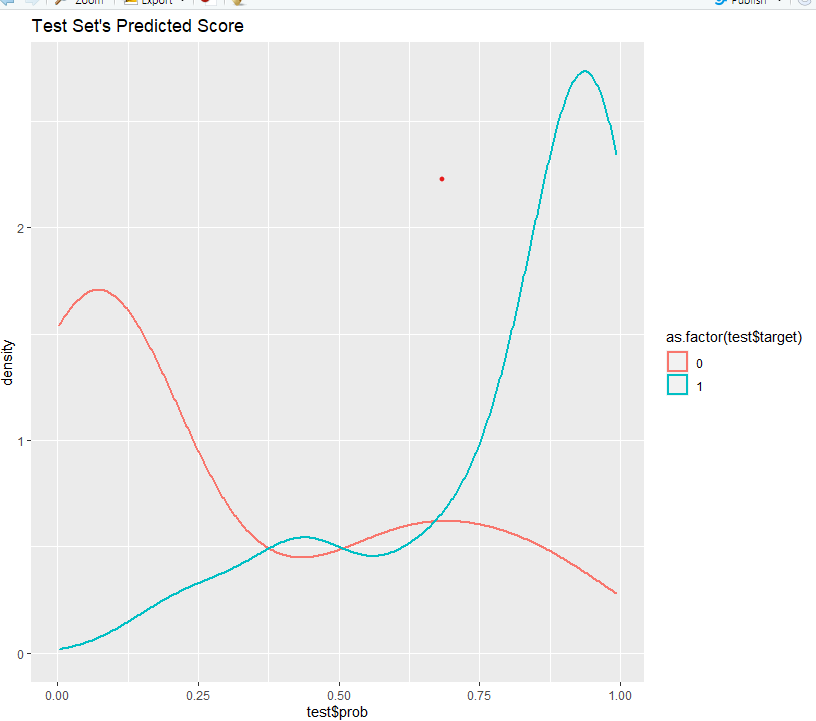
\includegraphics[width=1\textwidth]{task1_1_testScore.png}
\end{figure}
The evaluation summary of logistic regression can be seen below
\begin{lstlisting}[language=R]
  > Confusion
         Actual
Predicted  0  1
        0 31  7
        1 14 37
> AccuracyRate
[1] 0.7640449
> plot(rocCurve)
> rocCurve$sensitivities
[1] 1.0000000 0.6888889 0.0000000
> rocCurve$specificities
[1] 0.0000000 0.8409091 1.0000000
> rocCurve$au
Area under the curve: 0.7649
\end{lstlisting}

\subsection{method2}
\subsection{method3}
\subsection{discuss}


\section{Task2}
\subsection{Describe the Reuters-21578 corpus}
Reuters-21578 is a test collection for text classification research that is a multi-class, multi-label dataset. This dataset contains 90 classes, 7769 training files, and 3019 test files is a ModApte subdirectory of the Reuters-21578 benchmark. The Reuters-21578 dataset was originally collected and tagged by the Carnegie Group and Reuters in 1987 during the development of the CONSTRUE text classification system, and later by AT\&T Labs Research in September 1997. released in February, with David D. Lewis as the lead publisher

\subsection{Describe how each document is represented in your implementation.}
\begin{lstlisting}[language=R]
> data(Reuters21578)
> class(Reuters21578)
[1] "VCorpus" "Corpus" 
> head(Reuters21578)
<<VCorpus>>
Metadata:  corpus specific: 0, document level (indexed): 0
Content:  documents: 6
> summary(Reuters21578)
      Length Class             Mode
1     2      PlainTextDocument list
2     2      PlainTextDocument list
3     2      PlainTextDocument list
4     2      PlainTextDocument list
5     2      PlainTextDocument list
...
\end{lstlisting}

We import the Reuters-21578 as Vcorpus, which contains Metadata and Content. The metadata attribute contains author, datetime stamp, description, heading id, language, origin, lewissplit, cgisplit, oldid, topics\_cat, places, people, orgs, exchanges. The content is the raw data.

The data structure in the tm package that mainly manages documents is called Corpus, which represents a collection of documents. The corpus is divided into a dynamic corpus (Volatile Corpus) and a static corpus (Permanent Corpus). A dynamic corpus will be stored in memory as an R object and can be generated by either VCorpus() or Corpus(). The dynamic corpus, on the other hand, is stored as an R external file and can be generated using the PCorpus() function.

\subsection{Describe the whole procedure on applying LDA to this corpus to perform topic modeling.}
\begin{enumerate}
  \item Import the dataset
  \item Pre-processing the dataset, including transforming the content to lower case, striping whitespace, removing stopwords, punctuation and numbers, and steming document. 
  \item Calculate the BOW/TF-IDF document term matrix, ``bowdtm`` and ``tfidfdtm``
  \item Reducing the dimension with ``tfidfdtm``
  \item Calculate the word cloud with ``bowdtm``
  \item Apply LDA analysis.
\end{enumerate}

\subsection{Describe the parameter setting that you use in the LDA and explain their meanings.}
\begin{lstlisting}[language=R]
 result <- LDA(bowdtm, k, method="Gibbs", control=list(iter = 25, verbose = 25, alpha = 0.1))
\end{lstlisting}

\begin{itemize}
  \item ``bowdtm``: The document term matrix with BOW method.
  \item ``k``: number of topics
  \item ``method=Gibbs``: Applying Gibbs sampling
  \item ``control=list(iter = 25, verbose = 25, alpha = 0.1)``: inference via 25 iterations.
\end{itemize}

\subsection{Describe the output of your code and visualize the obtained topics in appropriate ways}
Draw the word cloud from the TF-IDF document term matrix
\begin{lstlisting}[language=R]
  > bowdtm <- bowdtm[slam::row_sums(bowdtm) > 0, ]
> k <- 20
> result <- LDA(bowdtm, k, method="Gibbs", control=list(iter = 25, verbose = 25, alpha = 0.1))
K = 20; V = 32697; M = 19042
Sampling 25 iterations!
Iteration 25 ...
Gibbs sampling completed!
> result
A LDA_Gibbs topic model with 20 topics.
> terms(result, 10)
      Topic 1   Topic 2   Topic 3   Topic 4    Topic 5   Topic 6   Topic 7   Topic 8      Topic 9    Topic 10  Topic 11  Topic 12  Topic 13  Topic 14 Topic 15 
 [1,] "said"    "said"    "said"    "said"     "dlrs"    "billion" "said"    "tonn"       "bank"     "said"    "said"    "oil"     "said"    "pct"    "said"   
 [2,] "govern"  "will"    "trade"   "trade"    "mln"     "bank"    "market"  "said"       "said"     "share"   "reuter"  "said"    "export"  "will"   "share"  
 [3,] "econom"  "compani" "japan"   "reuter"   "said"    "pct"     "rate"    "mln"        "debt"     "compani" "mine"    "price"   "will"    "issu"   "stock"  
 [4,] "japan"   "new"     "offici"  "futur"    "year"    "franc"   "dollar"  "wheat"      "loan"     "stock"   "gold"    "gas"     "produc"  "said"   "compani"
 [5,] "offici"  "reuter"  "state"   "price"    "quarter" "said"    "bank"    "export"     "billion"  "reuter"  "will"    "barrel"  "price"   "mln"    "inc"    
 [6,] "minist"  "car"     "import"  "pct"      "compani" "year"    "trade"   "reuter"     "dlrs"     "court"   "compani" "product" "coffe"   "bond"   "dlrs"   
 [7,] "year"    "trade"   "japanes" "new"      "sale"    "mln"     "analyst" "agricultur" "will"     "offer"   "ton"     "mln"     "reuter"  "dlrs"   "offer"  
 [8,] "will"    "motor"   "unit"    "cent"     "earn"    "reuter"  "currenc" "year"       "interest" "file"    "oper"    "compani" "meet"    "rate"   "will"   
 [9,] "west"    "exchang" "will"    "tonn"     "share"   "foreign" "dealer"  "grain"      "countri"  "board"   "ounc"    "dlrs"    "countri" "reuter" "reuter" 
[10,] "japanes" "market"  "reuter"  "contract" "report"  "mark"    "exchang" "crop"       "new"      "inc"     "power"   "will"    "quota"   "manag"  "common" 
      Topic 16  Topic 17  Topic 18  Topic 19 Topic 20  
 [1,] "said"    "said"    "said"    "mln"    "pct"     
 [2,] "tax"     "compani" "compani" "cts"    "year"    
 [3,] "billion" "dlrs"    "will"    "net"    "said"    
 [4,] "budget"  "reuter"  "reuter"  "loss"   "billion" 
 [5,] "bill"    "share"   "inc"     "dlrs"   "februari"
 [6,] "stg"     "mln"     "corp"    "shr"    "januari" 
 [7,] "hous"    "corp"    "system"  "reuter" "rose"    
 [8,] "dlrs"    "inc"     "new"     "profit" "rise"    
 [9,] "reuter"  "group"   "servic"  "rev"    "last"    
[10,] "bank"    "will"    "comput"  "oper"   "month"  
\end{lstlisting}

We should remove empty rows in ``bowdtm`` and set number of topics to 20. Then we can compute the LDA model, inferencing via 25 iterations of Gibbs sampling.

We can see the 10 most likely terms within the term probabilities beta of the inferred topics.

We took eight sample documents and get topic proportions form example documents.

\begin{lstlisting}
examples <- c(2, 100, 200, 400, 800, 1000, 1200, 1400)
lapply(pre_process_reuters[examples], as.character)

theta <- tmposterior$topics
N <- length(examples)

tpExamples <- theta[examples,]
colnames(tpExamples) <- nameOfTopics
vizDataFrame <- melt(cbind(data.frame(tpExamples), document = factor(1:N)), variable.name = "topic", id.vars = "document")  
vizDataFrame
\end{lstlisting}

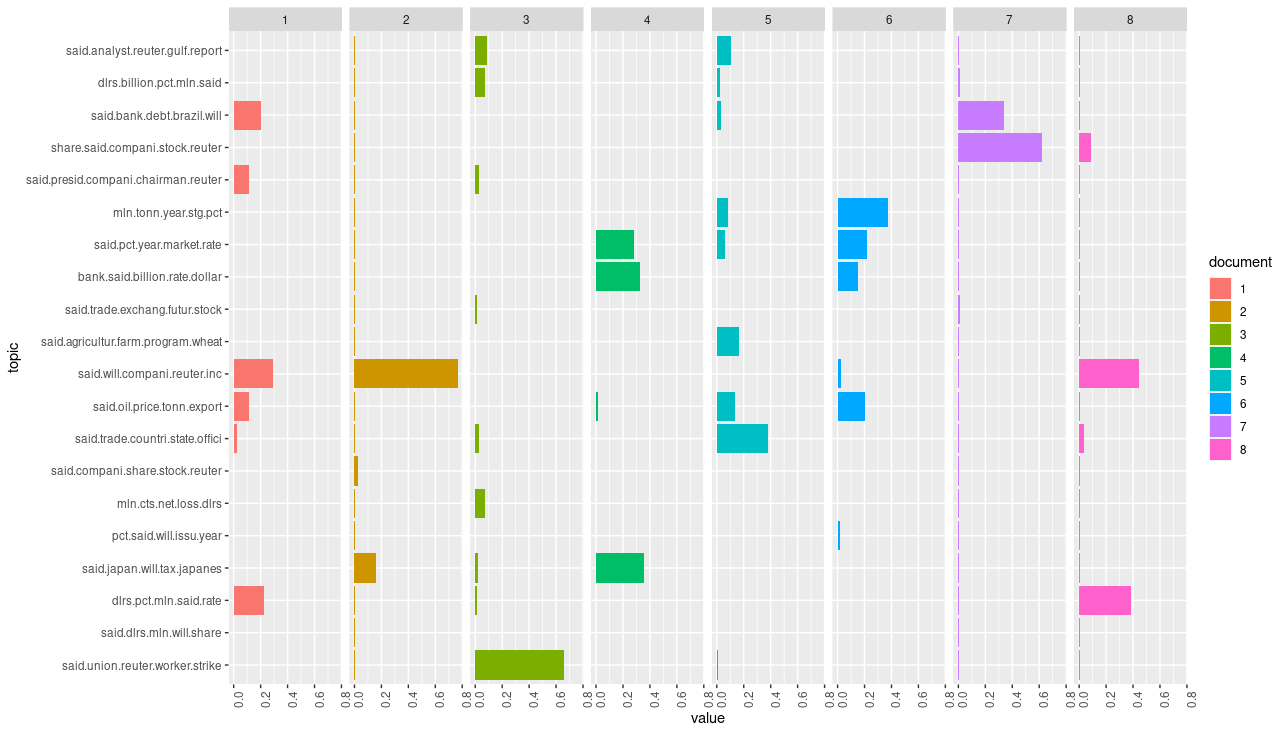
\includegraphics[width=.8\textwidth]{./task2.2.png}

\section{Task3}
\subsection{Data mining and cleaning}
This data comes from Twitter sentiment analysis in kaggle, From a data set of nearly one million, 13,700 comments about Alan bryd were selected. Among these data, 9,700 positive sentiment data. 4000 negative emotion data. In order to balance the data set, 4000 positive sentiment data and 4000 negative sentiment data were extracted.
 \begin{figure}[H]
\centering
  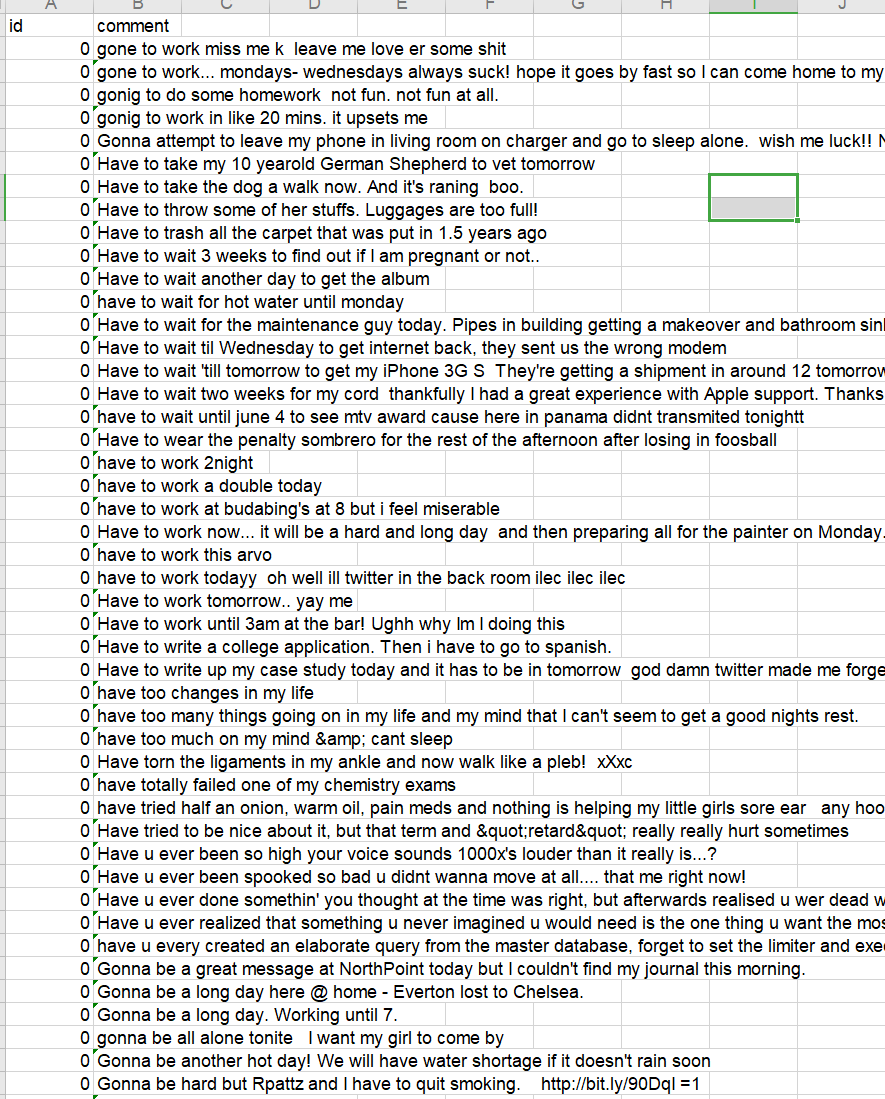
\includegraphics[width=1.0\textwidth]{3-1.png} %1.png是图片文件的相对路径

\end{figure}
There are most characters in the comments, such as emoji, @ other users and some garbled characters are inconsistent in capitalization
 \begin{figure}[H]
\centering
  
\includegraphics[width=.8\textwidth]{3-2.png} %1.png是图片文件的相对路径
  \end{figure}
So a series of data cleaning operations are used to clean the data.
 \begin{figure}[H]
\centering
  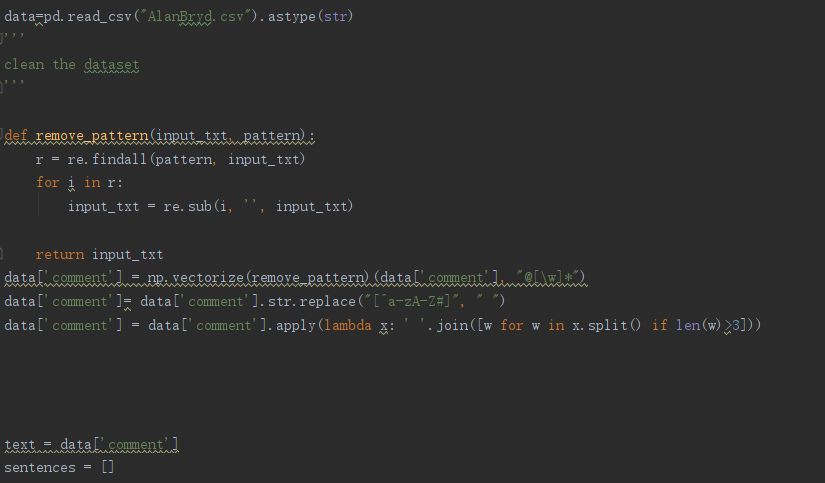
\includegraphics[width=.8\textwidth]{3-3.png} %1.png是图片文件的相对路径
  \end{figure}
\subsection{Use word2vec to build word vectors}
 \begin{figure}[H]
\centering
  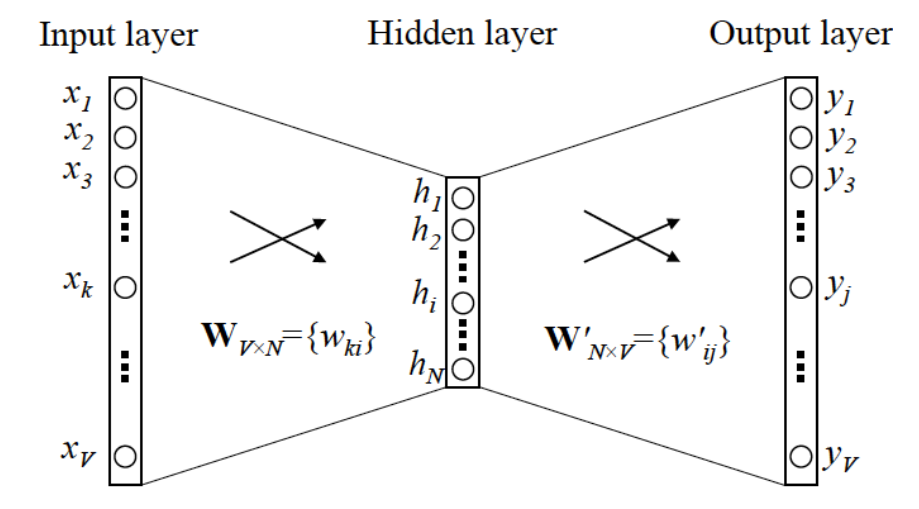
\includegraphics[width=.8\textwidth]{3-4.png} %1.png是图片文件的相对路径
  \end{figure}
Use word2vec's word vector for word embedding as input to the model
 \begin{figure}[H]
\centering
  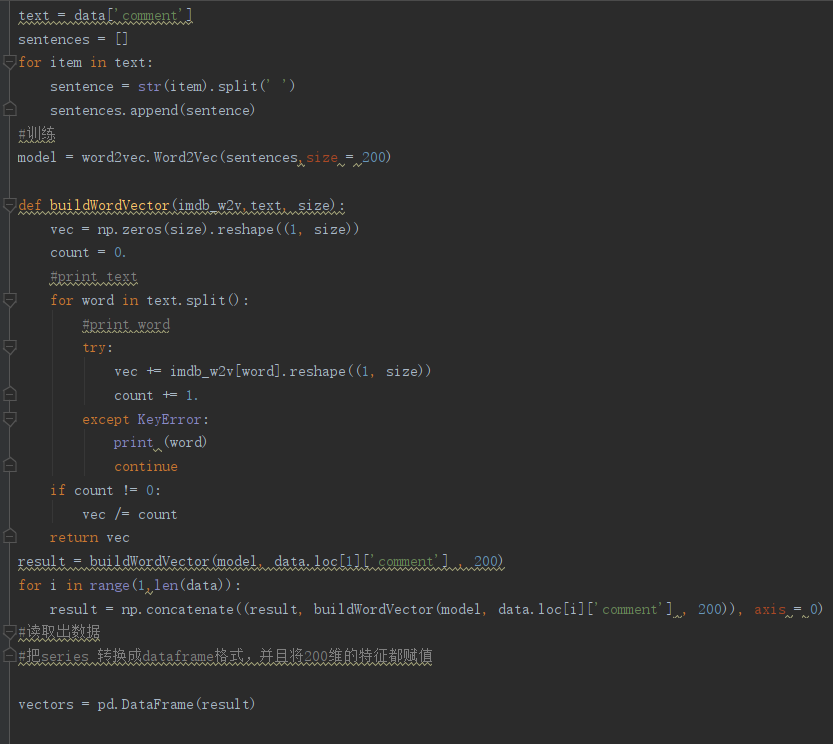
\includegraphics[width=.8\textwidth]{3-5.png} %1.png是图片文件的相对路径
  \end{figure}
\subsection{model using and result}
\subsubsection{GBDT}
theory of GBDT
 \begin{figure}[H]
\centering
  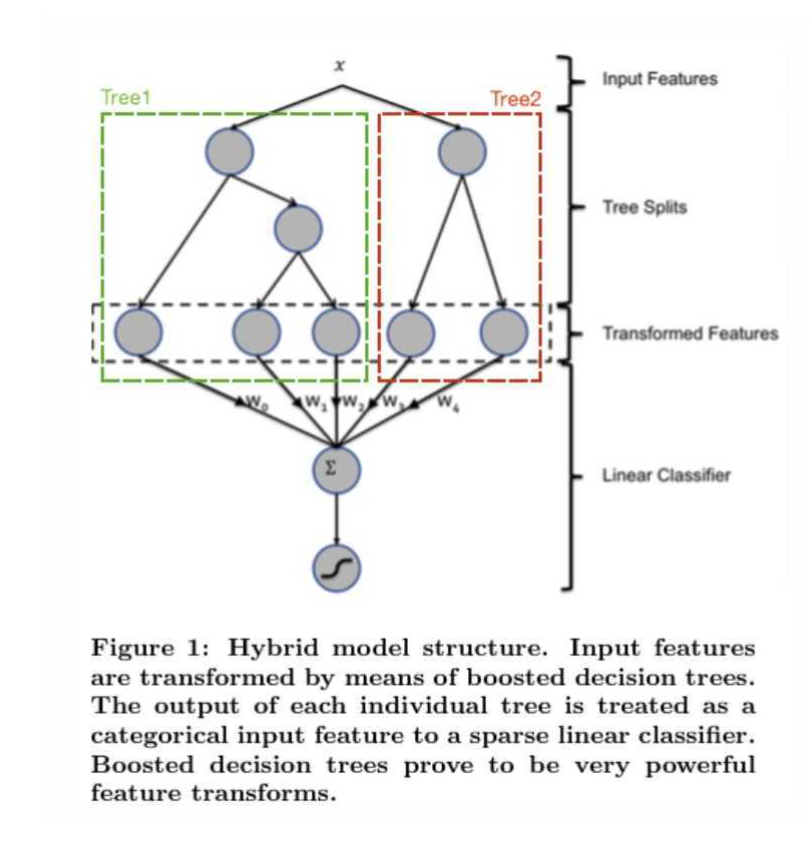
\includegraphics[width=.8\textwidth]{3-6.png} %1.png是图片文件的相对路径
  \end{figure}
Parameters of gbdt:\\
    $n_estimators=1000,$
    $subsample=0.8,$
    $loss='deviance',$
    $max_features='sqrt',$

  \subsubsection{SVM}
 theory of SVM
  \begin{figure}[H]
\centering
  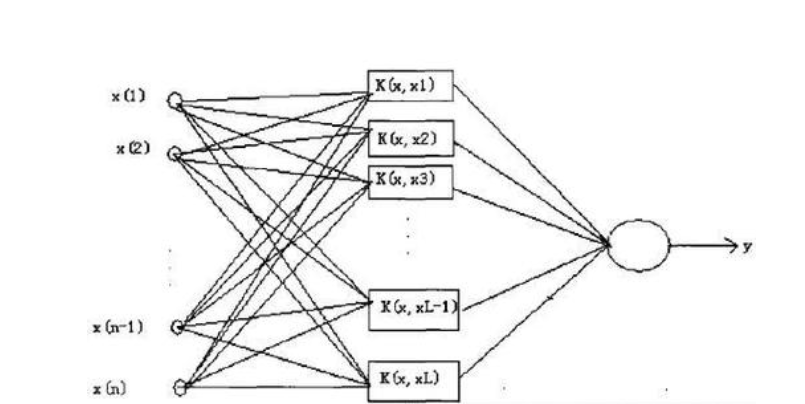
\includegraphics[width=.8\textwidth]{3-7.png} %1.png是图片文件的相对路径
  \end{figure}
Parameters of SVM:
$
kernel=‘rbf’
degree=3
$
\subsubsection{RandomForest}
 theory of RF
   \begin{figure}[H]
\centering
  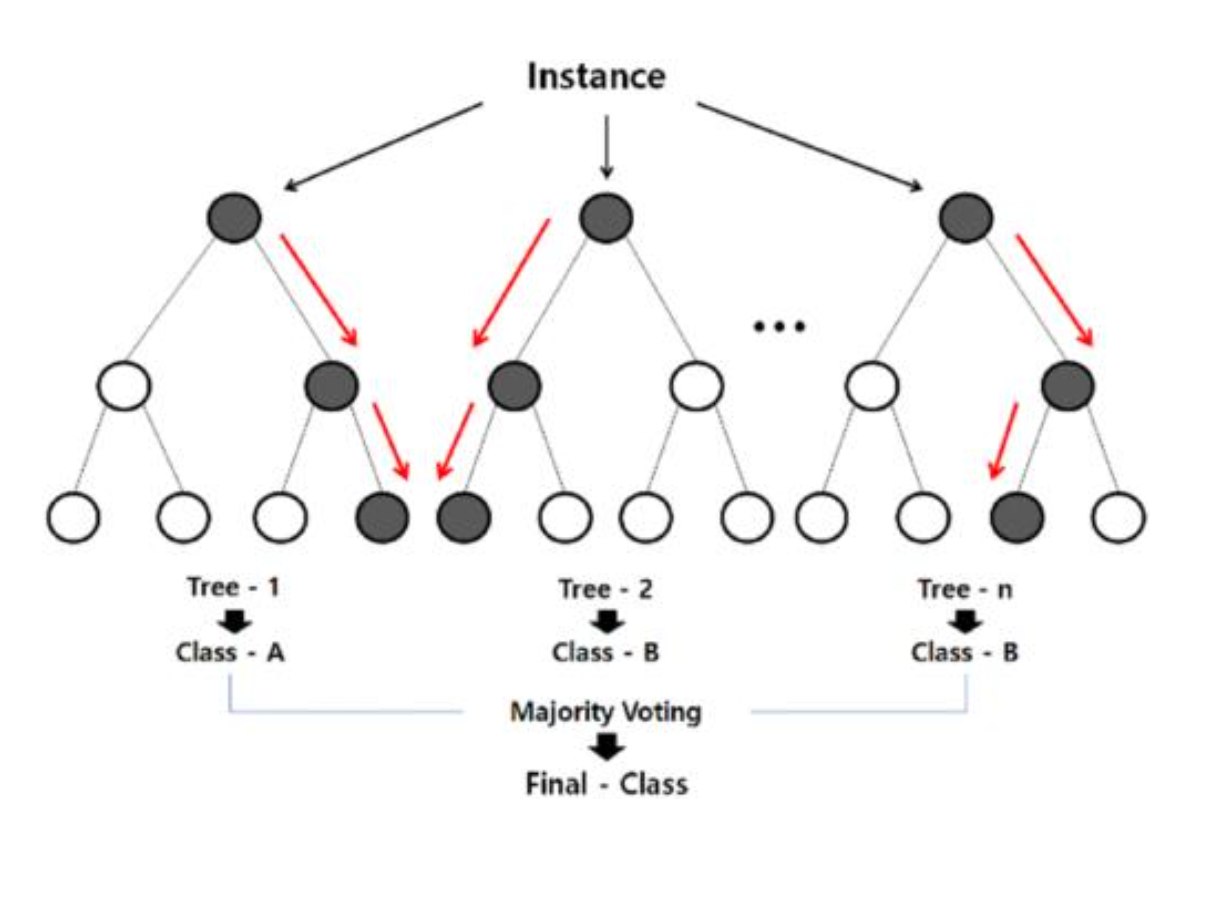
\includegraphics[width=.8\textwidth]{3-8.png} %1.png是图片文件的相对路径
  \end{figure}
Parameters of RF:$
    oob_score=True,
    n_estimators=400,
    max_features='sqrt',
    $
\subsubsection{ExtraTrees}
theory of ET
   \begin{figure}[H]
\centering
  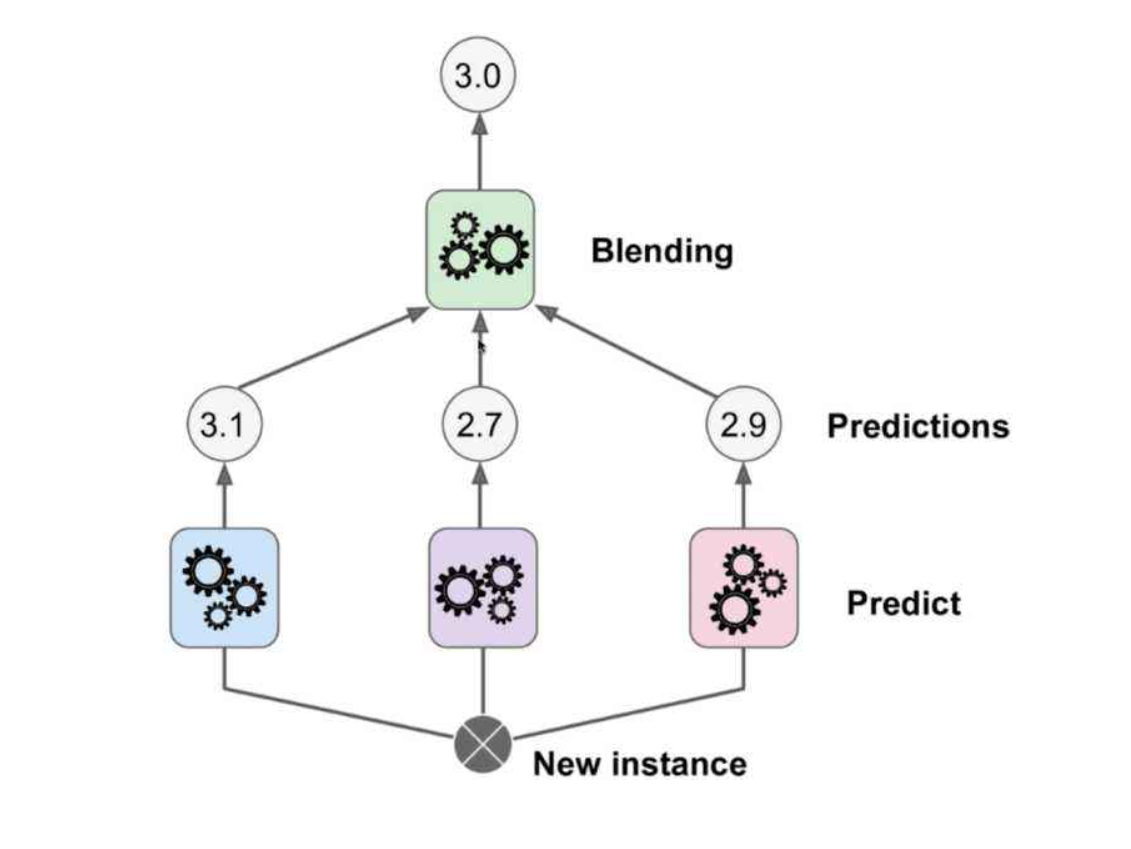
\includegraphics[width=.8\textwidth]{3-9.png} %1.png是图片文件的相对路径
  \end{figure}
 Parameter of ET:
 $
 criterion=gini,
 max features=log,
 max depth=50
 $
 \subsubsection{Result}
    \begin{figure}[H]
\centering
  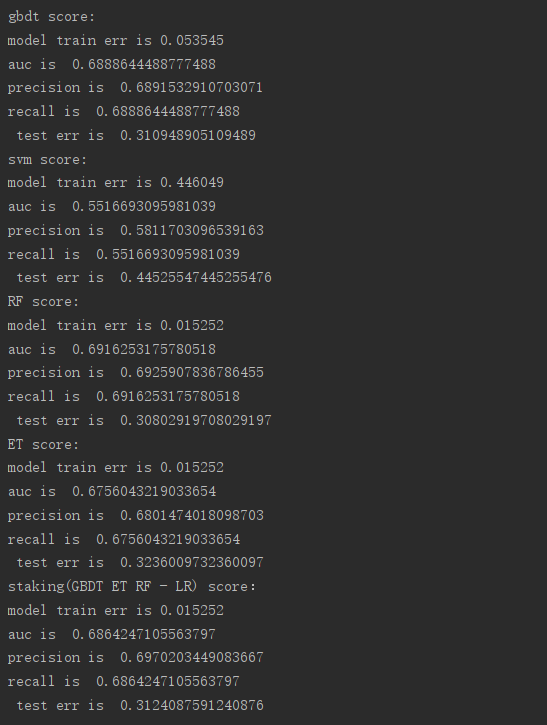
\includegraphics[width=.8\textwidth]{3-10.png} %1.png是图片文件的相对路径
  \end{figure}
According to the picture above,The expressive power of gbdt is better than other models in all aspects, and the mathematical model in machine learning can fit the features well when the data set is not large. Compared with other tree models, GBDT has a stronger ability to fit data by calculating residuals.
The auc figure of GBDT is :
    \begin{figure}[H]
\centering
  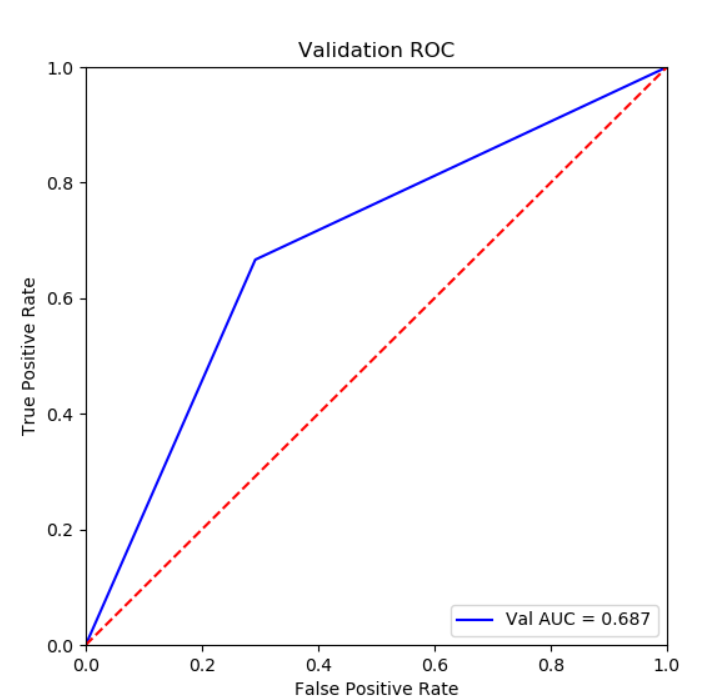
\includegraphics[width=.8\textwidth]{3-11.png} %1.png是图片文件的相对路径
  \end{figure}
\end{document}
